\section{Mehrstoffsysteme}

System besteht aus $r$ Komponenten (= Stoffen). Wir betrachten nur Systeme,
welche Mischprozesse zulassen. Gemischte Zustände sind Endzustände von
Mischprozessen. Der ungemischte Zustand kann beschrieben werden durch
$\sigma_i = (U_i,V_i,N_i)$ für $i=1,\dots,r$ und der gemischte Zustand ist
gegeben durch $\sigma = (U,V,N_1,\dots,N_r)$.

\subsection{Thermodynamik von Mischungen}

\begin{minipage}{0.25\textwidth}
    \centering
    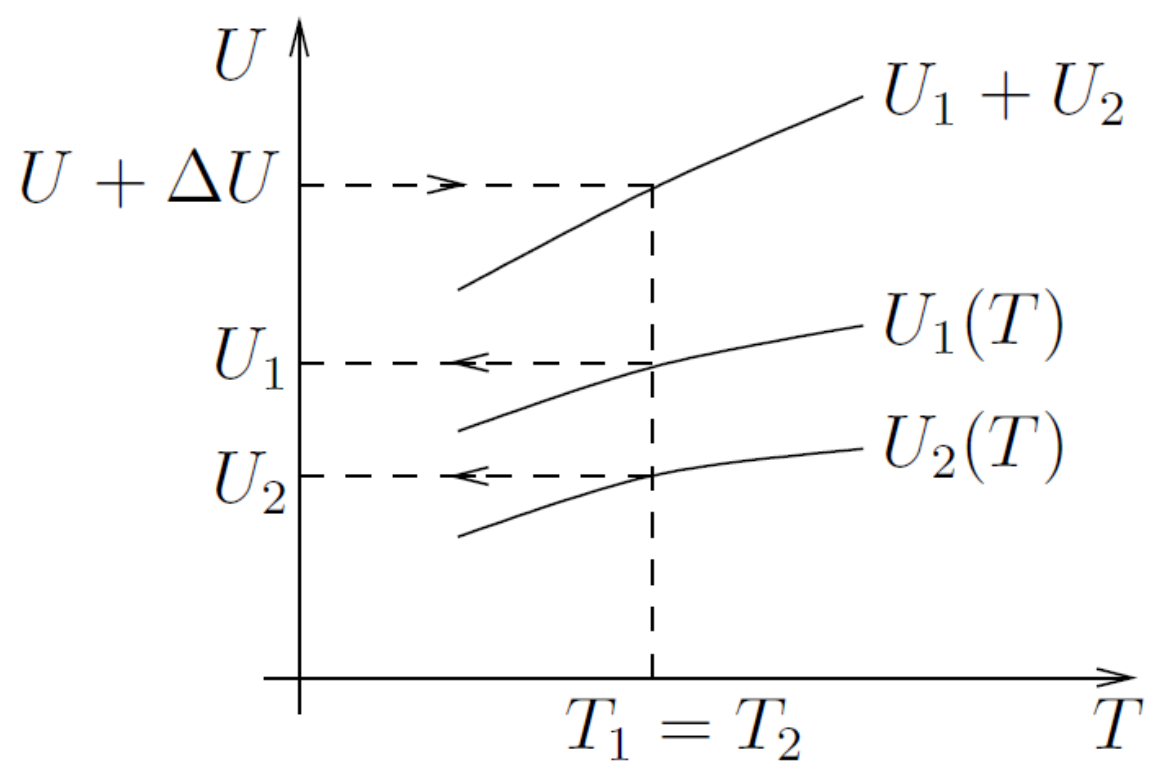
\includegraphics[width=\textwidth]{Bilder/Mehrstoffsystem_U.png}
\end{minipage}
\begin{minipage}{0.23\textwidth}
    Mischungen und Entmischungen werden durch semipermeable Wände realisiert.
    Diese Prozesse sind reversibel und kosten Arbeit. Sei $S = S_1 \vee S_2$ und
    $\Delta U$ die zugeführte Arbeit. Dann gilt:
\end{minipage}

\begin{align*}
    S_S (U,V,N_1,N_2) &= S_{S_1} (U_1,V,N_1) + S_{S_2} (U_2,V,N_2)
    \\
    U_1 + U_2 &= U + \Delta U
    \\
    T_1 &= T_2
\end{align*}
Nun können wir bereits bekanntes verallgemeinern:
\begin{align*}
    dS = \frac{1}{T} d U + \frac{p}{T} dV - \sum_{i=1}^r \frac{\mu_i}{T} d N_i
\end{align*}
Mit $p$ dem Gesamtdruck des Gemisches und $\mu_i$ den entsprechenden
chemischen Potentialen.
\begin{align*}
    \mu_i = - T \frac{\partial S}{\partial N_i} \Big|_{U,V,N_{j \neq i}}
\end{align*}
Von den $r+2$ intensiven Grössen $(T,p,\mu_1,\dots,\mu_r)$ sind nur $r+1$
frei wählbar. Insbesondere sind die $\mu_i$ intensiv und die $N_i$ extensiv.
Die chemischen Potentiale hängen nur von den Verhältnissen der $N_i$ ab:
\begin{align*}
    \mu_i = \mu_i(T,p,c_1,\dots,c_r)
    \hspace{10pt} , \hspace{10pt}
    c_i := \frac{N_i}{N}
    \hspace{10pt} , \hspace{10pt}
    N = N_1 + \dotsb + N_r
\end{align*}
Wegen $c_1 + \dotsb + c_r = 1$ sind nur $r-1$ Konzentrationen frei wählbar.
Die Gibbs'sche Phasenregel besagt neu
\begin{align*}
    f = r+2-n
\end{align*}

\paragraph{Extremalprinzip der Gibbs'schen Energie}
Da $G(T,p,N_1,\dots,N_r)$ konkav ist in $(T,p)$ und konvex in $(N_1,\dots,N_r)$
gilt:
\begin{align*}
    G'(T,p,N_1',\dots,N_r') + G'' (T,p,N_1'',\dots,N_r'') 
    \\ \geq
    G(T,p,N_1' + N_1'' ,\dots, N_r' + N_r'')
\end{align*}
Es folgt, dass im Gleichgewicht gilt: $\mu_i' = \mu_i''$.

\subsection{Ideale Mischungen}

Ideale Mischungen sind charakterisiert durch $\Delta U = 0$ und somit
\begin{align*}
    U = \sum_{i=1}^r U_i
\end{align*}
wobei $U_i = U_i (U,V,N_1,\dots,N_r)$. Weiter gilt $T_i = T_j \ \forall
i,j =1,\dots,r$ und
\begin{align*}
    S(U,V,N_1,\dots,N_r) = \sum_{i=1}^r S_i (U_i,V,N_i)
\end{align*}
Für ideale Mischungen ist die adiabatische Entmischung isotherm.
\begin{align*}
    \frac{1}{T} = \frac{\partial S}{\partial U} \Big|_{V,\geschwungeneklammer{N_k}}
    = \sum_{i=1}^r \frac{\partial S_i}{\partial U_i} \Big|_{V,N_i}
        \frac{\partial U_i}{\partial U} \Big|_{V,\geschwungeneklammer{N_k}}
    = \frac{1}{T_1} \sum_{i=1}^r \frac{\partial U_i}{\partial U} \Big|_{V,\geschwungeneklammer{N_k}}
    = \frac{1}{T_1}
\end{align*}
mit $T_1 \equiv T_i \ \forall i$ und $T$ der Temperatur des Mischung.
Für die Freie Energie gilt:
\begin{align*}
    F(T,V,N_1,\dots,N_r) = U - T S
    = \sum_{i=1}^r U_i - T \sum_{i=1}^r S_i
    = \sum_{i=1}^r F_i (T,V,N_i)
\end{align*}
Somit:
\begin{align*}
    p = - \frac{\partial F}{\partial V} \Big|_{T,N_i}
    = - \sum_{i=1}^r \frac{\partial F_i}{\partial V} \Big|_{T,N_i}
    = \sum_{i=1}^r p_i
\end{align*}
Mit $p_i$ den Partialdrücken. Dass die Summe der Partialdrücke den Gesamtdruck
der Mischung ergibt ist bekannt unter dem Namen Daltons Gesetz. Weiter gilt:
\begin{align*}
    G(T,p,N_1,\dots,N_r)
    = \sum_{i=1}^r U_i - T \sum_{i=1}^r S_i + V \sum_{i=1}^r p_i
    = \sum_{i=1}^r G_i (T,p_i,N_i)
\end{align*}
Daraus folgt:
\begin{align*}
    \frac{\partial G_i}{\partial p_i} \Big|_{T,N_i}
    &= \frac{\partial G}{\partial p} \Big|_{T,N_i}
    = V
    \\
    \frac{\partial G}{\partial N_i} \Big|_{T,p,N_{j \neq i}}
    &= \mu_i (T,p,N_1,\dots,N_r)
\end{align*}
Hier ist $\mu_i$ das chemische Potential der $i$-ten Komponente in der
Mischung. Für gegebenes $p$ und $T$ gilt $G_i (T,p_i,N_i) = G_i (T,p_i(N_1,\dots,N_r),N_i)$
und somit:
\begin{align*}
    \mu_i (T,p,N_1,\dots,N_r)
    = \mu_i^0 (T,p_i)
\end{align*}
wobei $\mu_i^0$ das chemische Potential des reinen Stoffes ist.
Im Falle eines idealen Gases gilt:
\begin{align*}
    \frac{\partial G}{\partial p} \Big|_{T,N} = V = \frac{N R T}{p}
\end{align*}
und somit:
\begin{align*}
    G_i(T,p_i,N_i) &= G_i (T,p,N_i) + \int_{p}^{p_i} \frac{\partial G_i}{\partial p'} \Big|_{T,N_i} dp'
    \\
    &= G_i (T,p,N_i) + N_i R T \log \klammer{\frac{N_i}{N}}
    \\
    \Rightarrow
    G(T,p,N_1,\dots,N_r) &= \sum_{i=1}^r G_i (T,p,N_i) + N_i R T \log \klammer{\frac{N_i}{N}}
\end{align*}
Weiter gilt:
\begin{align*}
    \mu_i(T,p,N_1,\dots,N_r) = \frac{\partial G}{\partial N_i} \Big|_{T,p}
    &= \underbrace{\frac{\partial G_i}{\partial N_i} \Big|_{T,p}}_{=\mu_i^0 (T,p)}
        + R T \log \klammer{\frac{N_i}{N}}
    \\
    &= \mu_i^0 (T,p) + R T \log(c_i)
\end{align*}
Mit $\frac{p_i}{p} = \frac{N_i}{N} = c_i$ den Konzentrationen.
Weiter folgt:
\begin{align*}
    S(T,p,N_1,\dots,N_r) = - \frac{\partial G}{\partial T} \Big|_{p,N_i}
    = \sum_{i=1}^r S_i(T,p,N_i) - R \sum_{i=1}^r N_i \log \klammer{\frac{N_i}{N}}
\end{align*}
Der Term $- R \sum_{i=1}^r N_i \log \klammer{\frac{N_i}{N}} > 0$ wird
Mischentropie genannt.

\subsection{Verdünnte Mischung}

In Fällen wo die Potentiale der gemischten Zustände vereinfacht geschrieben werden
kann sind verdünnte Mischungen. Im folgenden soll Stoff $1$ ein Lösungsmittel sein
mit Konzentration $c_1 \approx 1$ und $c_i \ll 1 \ \forall i = 2,\dots,r$. Wir nehmen
an dass $U$ und $V$ bei festem $T$ und $p$ linearisiert werden können.
\begin{align*}
    U(T,p,N_1,\dots,N_r) &= N_1 U \klammer{T,p,1,\frac{N_2}{N_1},\dots,\frac{N_r}{N}}
    \\
    &\approx N_1 \klammer{\tilde{u}_1 (T,p) + \sum_{i=2}^r \frac{N_i}{N_1} \tilde{u}_1 (T,p)}
    \\
    &= \sum_{i=1}^r N_i \tilde{u}_i (T,p)
    \\
    V(T,p,N_1,\dots,N_r) &\approx \sum_{i=1}^r N_i \tilde{v}_i (T,p)
\end{align*}
Hier ist $\tilde{u}_i = \frac{U_i}{N_i}$ die spezifische Energie und $\tilde{v}_i
= \frac{V_i}{N_i}$ das spezifische Volumen. Nun haben wir ein hypothetisches System
sodass:
\begin{align*}
    \tilde{U} = \sum_{i=1}^r N_i \tilde{u}_i
    \hspace{10pt} , \hspace{10pt}
    \tilde{V} = \sum_{i=1}^r N_i \tilde{v}_i
\end{align*}
Für fixes $\vec{N} = (N_1,\dots,N_r)$ ist die Entropie ein exaktes Differential.
\begin{align*}
    d \tilde{S} = \frac{1}{T} \klammer{d \tilde{U} + p d \tilde{V}}
    = \sum_{i=1}^r N_i \frac{1}{T} \klammer{d \tilde{u}_i + p d \tilde{v}_i}
    = \sum_{i=1}^r N_i d \tilde{s}_i^0
\end{align*}
Also existiert eine Funktion $\tilde{s}_i^0 (\tilde{u}_i,\tilde{v}_i)$ so dass
\begin{align*}
    \tilde{S}(\tilde{U},\tilde{V},N_1,\dots,N_r)
    = \sum_{i=1}^r N_i \tilde{s}_i^0 (\tilde{u}_i,\tilde{v}_i) - R \sum_{i=1}^r N_i \log \klammer{\frac{N_i}{N}}
\end{align*}
Weiter gilt:
\begin{align*}
    \tilde{G}(T,p,N_1,\dots,N_r) =
    \sum_{i=1}^r N_i \tilde{\mu}_i^0(T,p) + R T N_i \log \klammer{\frac{N_i}{N}}
\end{align*}
mit $\tilde{\mu}_i^0 (T,p) := \tilde{u}_i(T,p) - T \tilde{s}_i^0 (T,p) + p \tilde{v}_i (T,p)$.
Es gilt:
\begin{align*}
    \tilde{\mu}_i (T,p,c_1,\dots,c_r) = \tilde{\mu}_i^0 (T,p) + R T \log(c_i)
\end{align*}
und
\begin{align*}
    \frac{\partial \tilde{\mu}_i}{\partial T} \Big|_p = - \tilde{s}_i^0 + R \log(c_i)
    \hspace{10pt} &, \hspace{10pt}
    \frac{\partial \tilde{\mu}_i}{\partial p} \Big|_T = \tilde{v}_i
    \\
    \frac{\partial \tilde{\mu}_i^0}{\partial T} \Big|_p = - \tilde{s}_i^0
    \hspace{10pt} &, \hspace{10pt}
    \frac{\partial \tilde{\mu}_i^0}{\partial p} \Big|_T = \tilde{v}_i
\end{align*}
Wenn $c_i \ll c_1 \ \forall i = 2,\dots,r$, dann $\log(c_1) \approx - \sum_{i=2}^r c_i$
und wir können schreiben:
\begin{align*}
    \mu_1 (T,p,c_1,\dots,c_r) = \tilde{\mu}_1^0 (T,p) - R T \sum_{i=2}^r c_i
\end{align*}

\subsection{Anwendungen}

\begin{minipage}{0.3\textwidth}
    \subsubsection{Osmotischer Druck}

    Betrachte eine feste semipermeable Wand die nur Stoff $1$ und Energie
\end{minipage} \hspace{5pt}
\begin{minipage}{0.175\textwidth}
    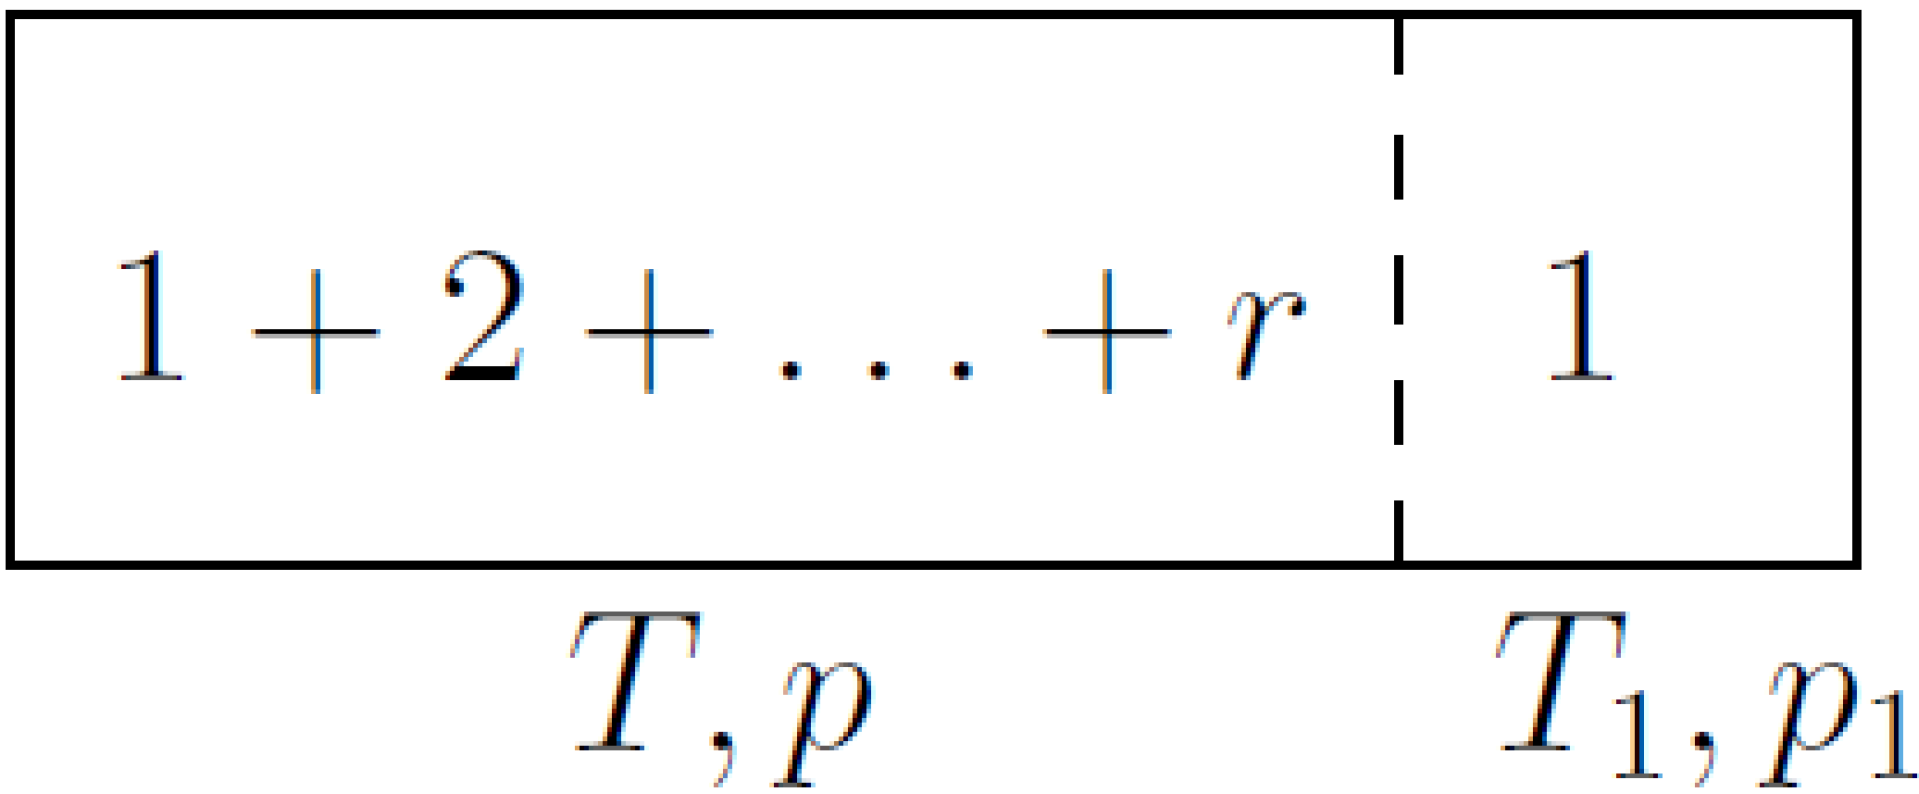
\includegraphics[width=\textwidth]{Bilder/Osmotischer_Druck.png}
\end{minipage}
austauschen lässt.
Gleichgewichtsbedingung: $T = T_1$ und $\mu_1 (T,p,c_1,\dots,c_r) = \mu_1^0 (T,p_1)$.
Wir nehmen an $c_i \ll c_1 \ \forall i = 2,\dots,r$ und $c_1 \approx 1$.
\begin{align*}
    \tilde{\mu}_1^0 (T,p) - \mu_1^0 (T,p_1) = R T \sum_{i=2}^r c_i
    \approx
    \mu_1^0 (T,p) - \mu_1^0 (T,p_1)
\end{align*}
Nach Linearisieren:
\begin{align*}
    \frac{\partial \mu_1^0}{\partial p} \Big|_T (p-p_1)
    = v_1 (p-p_1)
    = R T \sum_{i=2}^r c_i
\end{align*}
Für den osmotischen Druck $p-p_1$ folgt:
\begin{align*}
    p - p_1 = \frac{R T \sum_{i=2}^r c_i}{v_1}
\end{align*}

\subsubsection{Lösung eines idealen Gases}

\begin{minipage}{0.22\textwidth}
    Ein Gas ist gelöst in einer Flüssigkeit. Der Druck und die Temperatur sind fix.
\end{minipage} \hspace{5pt}
\begin{minipage}{0.25\textwidth}
    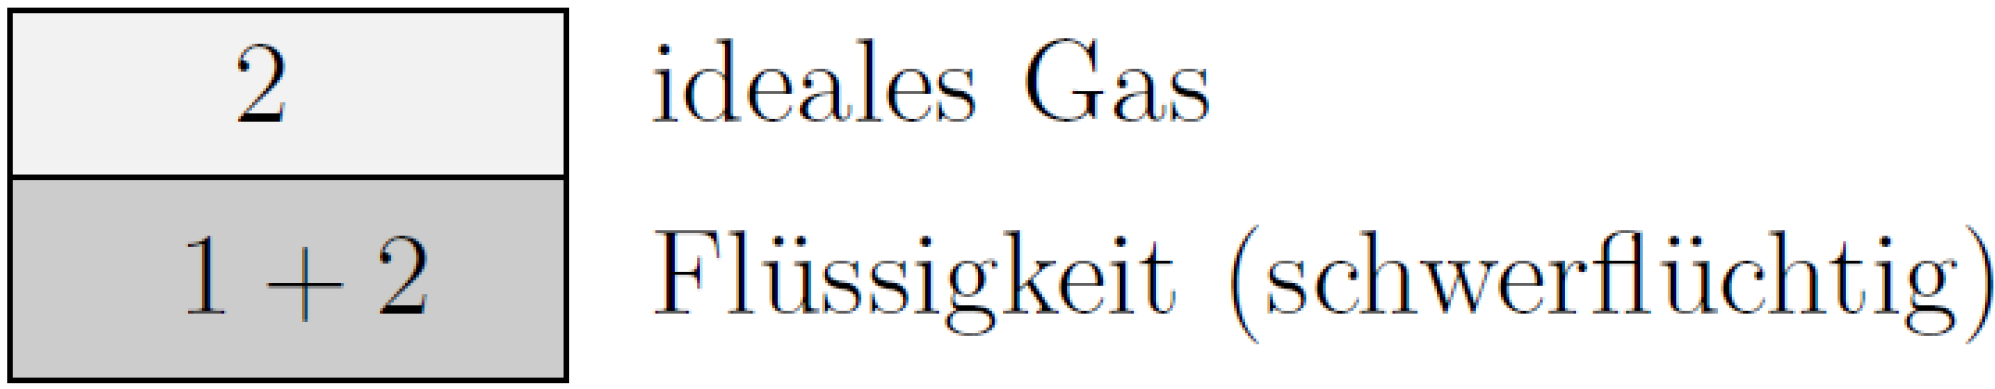
\includegraphics[width=\textwidth]{Bilder/Loesung_ideales_gas.png}
\end{minipage}

Für $\overline{\mu}_2^0$ dem chemischen Potential der reinen Gasphase und $\mu_2$
demjenigen der Mischung gilt:
\begin{align*}
    \mu_2 (T,p) = \overline{\mu}_2^0 (T,p) = \tilde{\mu}_2^0 (T,p) + R T \log(c_2)
    \\
    \frac{\partial \overline{\mu}_2^0}{\partial p} \Big|_T = \overline{v}_2
    \stackrel{\text{id. Gas}}{=} \frac{R T}{p}
    \hspace{10pt} , \hspace{10pt}
    \frac{\partial \tilde{\mu}_2^0}{\partial p} \Big|_T = \tilde{v}_2
\end{align*}
Hier sind $\overline{v}_2$ das Molvolumen des idealen Gases und $\tilde{v}_2$ die
Änderung des Lösungsvolumens bei der Lösung eines Mols des Gases. Unter der Annahme
$\tilde{v}_2 \ll \overline{v}_2$ gilt $\overline{v}_2 - \tilde{v}_2 \approx \overline{v}_2$
und aus $\overline{v}_2 \approx R T \frac{\partial}{\partial p} \log(c_2)$ erhalten
wir das \fat{Henry-Gesetz}.
\begin{align*}
    \frac{\partial \log(c_2)}{\partial p} \Big|_T = \frac{1}{p} = \frac{d \log(p)}{dp}
    \hspace{10pt} \Rightarrow \hspace{10pt}
    c_2 = \text{const} \cdot p
\end{align*}

\subsubsection{Konzentrationsverhältnisse in zwei nicht mischbaren Lösungsmitteln}

Betrachte zwei nicht mischbare Lösungsmittel $1$ und $1^\star$ und Substanzen
$2,\dots,r$ die gelöst sind in den Lösungsmitteln. Gleichgewichtsbedingung:
$\tilde{\mu}_i^0 (T,p) + R T \log(c_i) = \tilde{\mu}_i^{\star 0} (T,p) + R T \log(\overline{c}_i)$
wobei die linke Seite das chemische Potential in der Lösungs $1$ ist und die rechte
Seite dasjenige in der Lösung $1^\star$ ist. Es folgt die \fat{Nernst-Gleichung}:
\begin{align*}
    \frac{\overline{c}_i}{c_i} = e^{\frac{\tilde{\mu}_i^0 - \tilde{\mu}_i^{\star 0}}{R T}}
\end{align*}

\subsubsection{Phasengleichgewicht binärer Systeme}

\begin{figure}[h]
    \centering
    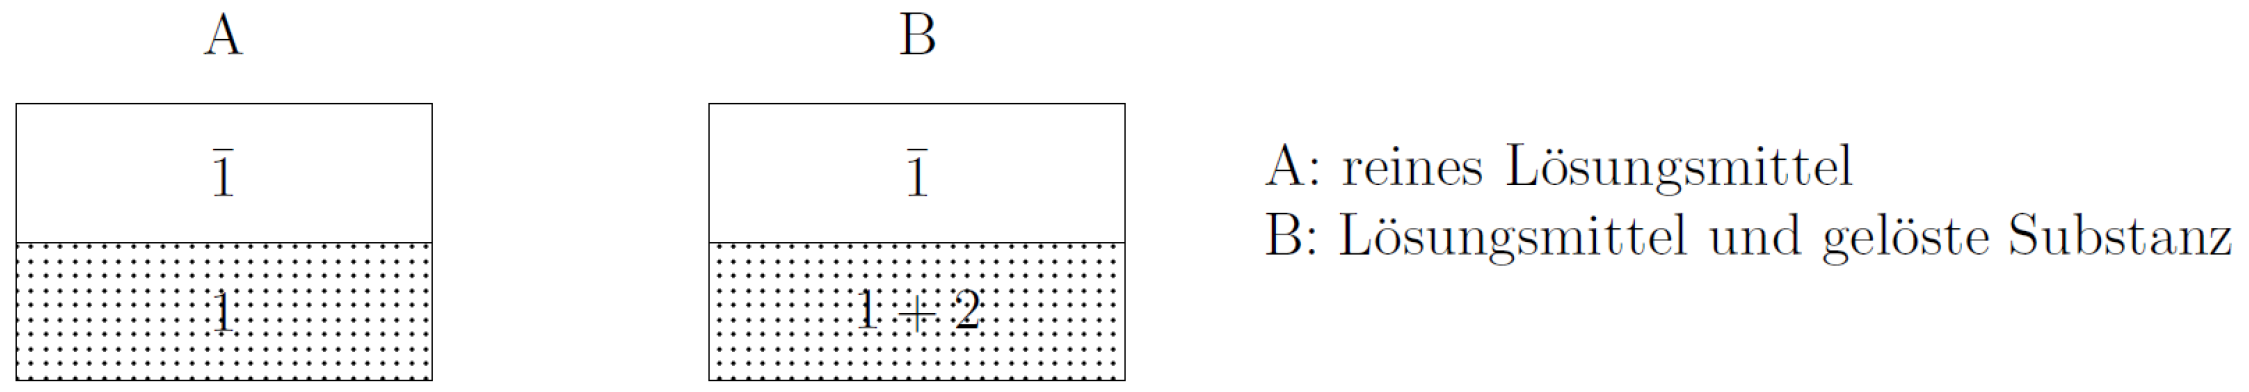
\includegraphics[width=0.48\textwidth]{Bilder/Phasengleichgewicht_binaere_Systeme.png}
\end{figure}

Gleichgewichtsbedingung: $\overline{\mu}_1^0 (T,p) = \mu_1 (T,p)$. Wobei
$\overline{\mu}_1^0 (T,p)$ das chemische Potential der ersten Substanz in Phase
$\overline{1}$ ist und $\mu_1 (T,p)$ das von der reinen Phase $1$ (A) respektive der
Lösung $1+2$ (B) bezeichnet. Nach Linearisierung:
\begin{align*}
    \overline{\mu}_1^0 (T^\ast,p^\ast) = \mu_1^0 (T,p) \hspace{10pt} (A)
    \hspace{10pt} , \hspace{10pt}
    \overline{\mu}_1^0 (T,p) = \mu_1^0 (T,p) - R T c_2 \hspace{10pt} (B)
\end{align*}
wobei $T^\ast$ und $p^\ast$ die Temperatur und der Druck sind wo der erste Stoff ohne
das Lösungsmittel im Gleichgewicht ist. Weiter gilt:
\begin{align*}
    \frac{\partial \mu_1^0}{\partial p} \Big|_T = v_1
    \hspace{10pt} , \hspace{10pt}
    \frac{\partial \mu_1^0}{\partial T} \Big|_p = - s_1
    \hspace{10pt} , \hspace{10pt}
    \frac{\partial \overline{\mu}_1^0}{\partial p} \Big|_T = \overline{v}_1
    \hspace{10pt} , \hspace{10pt}
    \frac{\partial \overline{\mu}_1^0}{\partial T} \Big|_p = - \overline{s}_1
\end{align*}
Mit $\Delta p = p - p^\ast$ und $\Delta T = T-T^\ast$ gilt:
\begin{align*}
    \mu_1^0 (T^\ast + \Delta T,p^\ast + \Delta p) &= \mu_1^0 (T^\ast,p^\ast) + v_1 \Delta p - s_1 \Delta T
    \\
    \overline{\mu}_1^0 (T^\ast + \Delta T,p^\ast + \Delta p) &= \overline{\mu}_1^0 (T^\ast,p^\ast) + \overline{v}_1 \Delta p - \overline{s}_1 \Delta T
    \\
    \Rightarrow \overline{\mu}_1^0 - \mu_1^0 &= (\overline{v}_1 - v_1) \Delta p - (\overline{s}_1 - s_1) \Delta T
    \\
    \Rightarrow - R T c_2 &= (\overline{v}_1 - v_1) \Delta p - (\overline{s}_1 - s_1) \Delta T
\end{align*}
Für $c_2 = 0$ erhalten wir die Clausius-Clepeyron Gleichung.
\begin{itemize}
    \item \underline{Dampfdruckniedrigung} ($\Delta T = 0$). Raoultsches Gesetz:
        \begin{align*}
            \Delta p = - \frac{R T c_2}{\overline{v}_1 - v_1}
        \end{align*}
    \item \underline{Siedepunktserhöhung / Gefrierpunktsniedrigung} ($\Delta p = 0$).
        \begin{align*}
            \Delta T = \frac{R T c_2}{\overline{s}_1 - s_1} = \frac{R T^2 c_2}{L_{1\overline{1}}}
        \end{align*}
        wobei $L_{1 \overline{1}}$ die Übergangswärme ist.
\end{itemize}

\subsection{Chemische Gleichgewichte}

Nun betrachten wir Reaktionen, bei denen sich die Stoffzahlen ändern können.
Seien $A_1,\dots,A_r$ die involvierten Stoffe die $s$ Reaktionen durchlaufen.
Es gilt:
\begin{align*}
    \sum_{i=1}^r \nu_i^k A_i
    \hspace{10pt} (k=1,\dots,s)
\end{align*}
mit $\nu_i^k \ \in \N$ den stöchiometrischen Koeffizienten

\begin{beispiel}
    Für $2 H_2 + O_2 \leftrightharpoons 2 H_2 O$ schreibt man
    $-2 H_2 - O_2 + 2 H_2 O = 0$ und somit $\nu = (-2,-1,2)$.
\end{beispiel}

Die Molzahlen $N_1,\dots,N_r$ können sich im materiell abgeschlossenen System
wie folgt verändern
\begin{align*}
    d N_i = \sum_{k=1}^s \nu_i^k d \lambda^k
    \hspace{10pt} \Rightarrow \hspace{10pt}
    N_i = N_i^0 + \sum_{k=1}^s \nu_i^k \lambda_i^k
\end{align*}
Hier ist $d \lambda^k$ der Grad bis zu dem die $k$-te Reaktion abgelaufen ist.
Falls $d \lambda^k = 1$ und $d \lambda^j = 0 \ \forall j \neq k$, erhalten
wir die Gleichgewichtsbedingung
\begin{align*}
    0 &= d G = \sum_{i=1}^r \frac{\partial G}{\partial N_i} d N_i
    = \vec{\nu} \cdot d \vec{N}
    = \sum_k \vec{\mu} \cdot \vec{\nu}^k d \lambda^k
    \\
    &\Rightarrow
    \sum_{i=1}^r \nu_i^k \mu_i = 0 \ \ \forall k = 1,\dots,s
\end{align*}

\begin{bemerkung}
    Es gilt:
    \begin{align*}
        G_i = N_i \mu_i = U_i - T S_i + p V_i
        \ \ \Rightarrow \ \
        \mu_i = u_i - T s_i + p v_i
    \end{align*}
    A priori können die Energie und die Entropie beliebig normiert sein.
    \begin{align*}
        u_i \mapsto u_i + a_i
        \hspace{10pt} , \hspace{10pt}
        s_i \mapsto s_i + b_i
        \hspace{10pt} \Rightarrow \hspace{10pt}
        \mu \mapsto \mu_i + a_i - b_i T =: \tilde{\mu}_i
    \end{align*}
    Die Normierungskonstanten müssen erfüllen:
    \begin{align*}
        \sum_{i=1}^r \nu_i^k (\mu_i + a_i - T b_i) = 0
        \hspace{10pt}
        k=1,\dots,s
    \end{align*}
\end{bemerkung}

\paragraph{Reaktionen in idealen Gasen}
Das chemische Potential der Komponenten im Gemisch:
\begin{align*}
    \mu_i (T,p,c_1,\dots,c_r) = \mu_i^0 (T,p) + R T \log(c_i)
\end{align*}
wobei $\mu_i^0(T,p)$ das chemische Potential der reinen Komponente bezeichnet.
Es folgt das \fat{Massenwirkungsgesetz}:
\begin{align*}
    \prod_{i=1}^r c_i^{\nu_i} =
    \exp \klammer{- \frac{1}{R T} \sum_i \nu_i \mu_i^0(T,p)}
    =: K(T,p)
\end{align*}
$K(T,p)$ hängt nur von $T$ und $p$ ab und bestimmt den Gleichgewichtszustand
$N_1,\dots,N_r$ auf der stöchiometrischen Geraden $N_i = N_i^0 + \lambda \nu_i$.

Wichtige Merkmale sind Volumenänderungen $\Delta V$ und Reaktionswärme $Q$.
Das Entfernen einer Wand bei festem $T$ und $p$ sind i.A. irreversibel. Nach
Einstellung des Gleichgewichts: $\Delta U = - p \Delta V + Q$. Mit
$H = p V + U$ folgt $Q = \Delta H$. Die Reaktion heisst endotherm, falls
$\Delta H > 0$ und exotherm, falls $\Delta H < 0$.

\subsubsection{Spezialfall: Ideale Gase}

Für ideale Gase sind innere Energie $U_i$ und Partialdrücke $p_i$ additiv.
\begin{align*}
    H(S,p,N_1,\dots,N_r) &= \sum_{i=1}^r H_i (S_i , p_i , N_i)
    \\
    H(T,p,N_1,\dots,N_r) &= \sum_{i=1}^r H_i(T,p_i,N_i) = \sum_{i=1}^r N_i h_i (T,p_i)
\end{align*}
Mit $h_i(T,p) = u_i(T) + p v_i(T,p) = u_i (T) + R T \equiv h_i(T)$.
\begin{align*}
    \Delta H &= \Delta \lambda \sum_{i=1}^r \nu_i h_i (T)
    \\
    \Delta V &= \Delta \lambda \sum_{i=1}^r \nu_i v_i (T,p)
        = \Delta \lambda \frac{R T}{p} \underbrace{\sum_{i=1}^r \nu_i}_{=: \nu}
\end{align*}
Hier ist $\nu$ die Anzahl der in der Reaktion gewonnenen/verlorenen Teilchen.
Für die $(T,p)$-Abhängigkeit des Gleichgewichts gilt wegen
\begin{align*}
    \frac{\partial \mu_i^0}{\partial p} \Big|_T = v_i
    \hspace{5pt} &, \hspace{5pt}
    \frac{\partial \mu_i^0}{\partial T} \Big|_p = - s_i
    \hspace{5pt} , \hspace{5pt}
    \frac{d h_i}{d T} = c_p^i (T)
\end{align*}
mit $c_p^i$ die isobare spezifische Wärme, dass
\begin{align*}
    \frac{\partial \log(K)}{\partial p} \Big|_T
    &= - \frac{1}{R T} \underbrace{\sum_{i=1}^r \nu_i v_i (T,p)}_{\Delta V}
    = - \frac{\nu}{p}
    \\
    \frac{\partial \log(K)}{\partial T} \Big|_p
    &= \frac{1}{R T^2} \sum_{i=1}^r \nu_i \underbrace{(\mu_i^0 + T s_i)}_{h_i = \Delta V}
    = \frac{\Delta H}{R T^2} = \frac{Q}{R T^2}
    \\
    \frac{\mathrm{d}}{\mathrm{d} T} \Delta H(T)
    &= \sum_{i=1}^r \nu_i c_p^i (T)
\end{align*}
Mit $\Delta V$ der Volumenänderung bei einmaligem Umsatz $\Delta \lambda = 1$ der
Reaktion. Für $\Delta V = 0,\nu=0$ ist $K$ unabhängig von $p$ und somit ist das
Gleichgewicht druckunabhängig. $\Delta H$ ist die Entropieänderung und Reaktionswärme
bei einmaligem Umsatz.

